\documentclass[handout, xcolor=dvipsnames,aspectratio=169]{beamer}
\usecolortheme[dark,accent=cyan]{solarized}
\usepackage[utf8]{inputenc}
\usepackage{multicol}
\usepackage{url}
\usepackage{hyperref}
\usepackage{subfig}
\title{Cryptography}
\author{Gaspare Ferraro}
\subtitle{A (nearly) complete overview}

\begin{document}

\begin{frame}[plain]
\maketitle
\begin{columns}
\column{0.5\textwidth}
	\center {
		
\includegraphics[width=0.3\textwidth]{style/qrcode.png}\\
		Visit us!\\
		\textcolor{solarizedCyan}{\href{https://zenhack.it}{zenhack.it}}
		}
\column{0.5\textwidth}
	\center{
		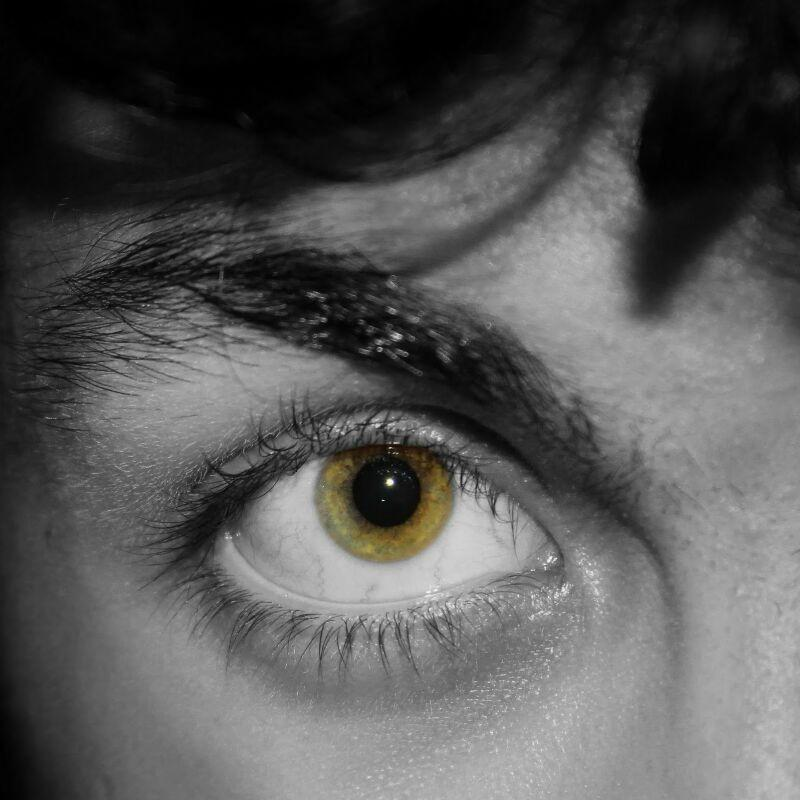
\includegraphics[width=0.3\textwidth]{style/gaspare.jpg}\\
		@GaspareG\\
		\textcolor{solarizedCyan}{ferraro@gaspa.re}
	}
	
\end{columns}
\end{frame}

%%%%%%%%%%%%%%%%%%%%%%%%%%%%%%%%%%%%%%%%%%%%%%%%%%%%%%%%%%%
\begin{frame}
  \centering
  \frametitle{Table of Contents}
  \begin{itemize}
    \item 1. Introduction
    \item 2. Message encoding
    \item 3. Classical cryptography
    \item 4. Symmetric-key cryptography
    \item 5. Public-key cryptography
    \item 6. Key exchange
    \item 7. Hash function
    \item 8. Steganography
  \end{itemize}  
\end{frame}
%%%%%%%%%%%%%%%%%%%%%%%%%%%%%%%%%%%%%%%%%%%%%%%%%%%%%%%%%%%
\begin{frame}
  \centering
  \frametitle{Table of Contents}
  \begin{itemize}
    \item 1. \textcolor{red}{Introduction}
    \item 2. Message encoding
    \item 3. Classical cryptography
    \item 4. Symmetric-key cryptography
    \item 5. Public-key cryptography
    \item 6. Key exchange
    \item 7. Hash function
    \item 8. Steganography
  \end{itemize}  
\end{frame}
%%%%%%%%%%%%%%%%%%%%%%%%%%%%%%%%%%%%%%%%%%%%%%%%%%%%%%%%%%%%%%%%%%%%%%%%%%%%%%%
\section[Section]{Introduction}
\part{Introduction}

%%%%%%%%%%%%%%%%%%%%%%%%%%%%%%%%%%%%%%%%%%%%%%%%%%%%%%%%%%%%%%%%%%%%%%%%%%%%%%%
\begin{frame}{Warning!}
  %\centering

  %In this lesson we will use \textcolor{red}{\textit{maths}}! 
  
  %\medskip

  %
\includegraphics[width=0.5\textwidth]{img/meme}

  %\medskip
  
  %It wasn't always like that though ...

\end{frame}

%%%%%%%%%%%%%%%%%%%%%%%%%%%%%%%%%%%%%%%%%%%%%%%%%%%%%%%%%%%%%%%%%%%%%%%%%%%%%%%
\begin{frame}{Why cryptography?}

\end{frame}

%%%%%%%%%%%%%%%%%%%%%%%%%%%%%%%%%%%%%%%%%%%%%%%%%%%%%%%%%%%%%%%%%%%%%%%%%%%%%%%
\begin{frame}{Cryptography yesterday}
    
  %\begin{figure}%
  %  \centering
  %  \subfloat[Cesare Chiper]{{
  %\centering
\includegraphics[width=5cm]{img/cesaer.png} }}%
  %  \qquad
  %  \subfloat[Scitala]{{
  %\centering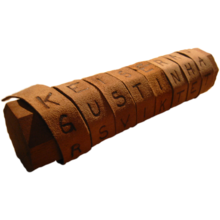
\includegraphics[width=5cm]{img/scitala.png} }}%
  %\end{figure}

\end{frame}

%%%%%%%%%%%%%%%%%%%%%%%%%%%%%%%%%%%%%%%%%%%%%%%%%%%%%%%%%%%%%%%%%%%%%%%%%%%%%%%
\begin{frame}{Cryptography today}
  %\center {
  %  The needs, as well as the resources available, have evolved
    
  %  and today we can divide cryptography into:

  %  \medskip
  %  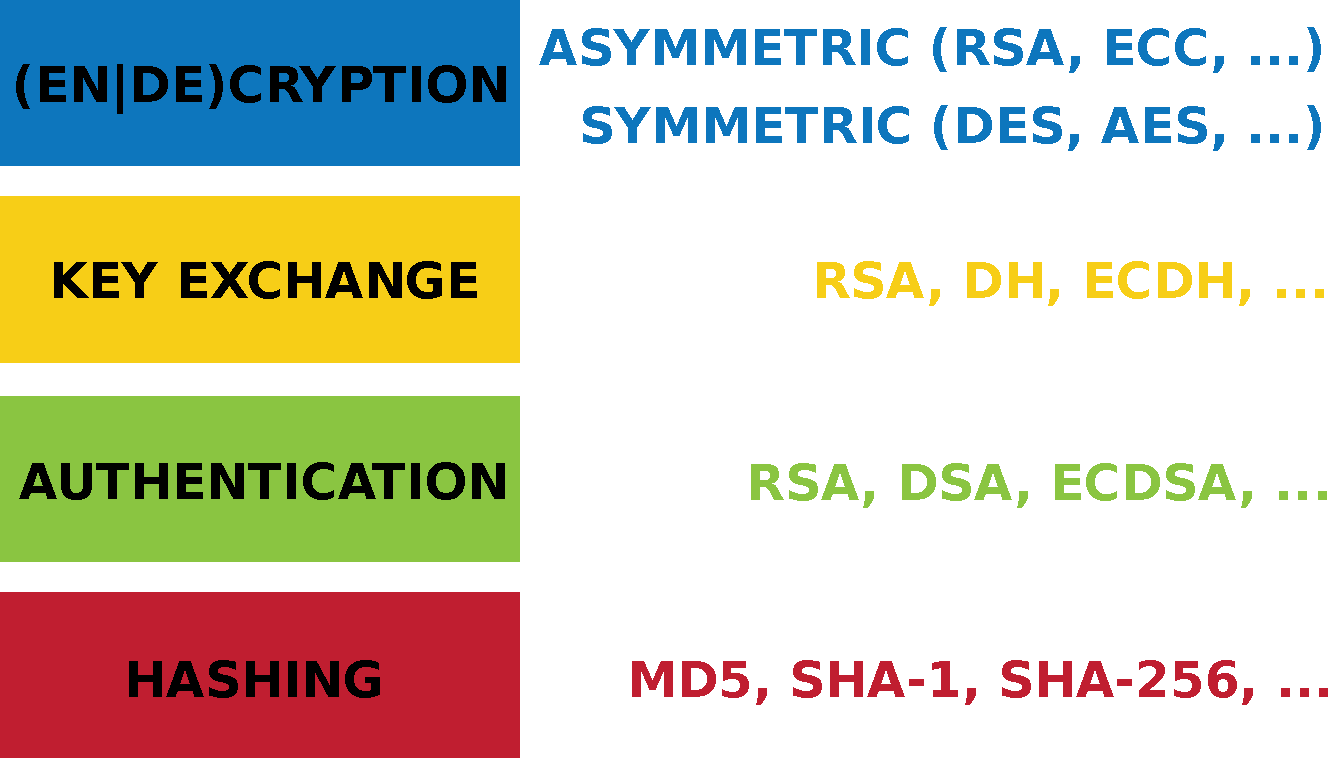
\includegraphics[width=0.6\textwidth]{include/crypto-section.pdf}
  %}
\end{frame}

%%%%%%%%%%%%%%%%%%%%%%%%%%%%%%%%%%%%%%%%%%%%%%%%%%%%%%%%%%%
\begin{frame}
  \centering
  \frametitle{Table of Contents}
  \begin{itemize}
    \item 1. Introduction
    \item 2. \textcolor{red}{Message encoding}
    \item 3. Classical cryptography
    \item 4. Symmetric-key cryptography
    \item 5. Public-key cryptography
    \item 6. Key exchange
    \item 7. Hash function
    \item 8. Steganography
  \end{itemize}  
\end{frame}
%%%%%%%%%%%%%%%%%%%%%%%%%%%%%%%%%%%%%%%%%%%%%%%%%%%%%%%%%%%%%%%%%%%%%%%%%%%%%%%
\section[Section]{Character encoding}
\part{Message and character encoding}

%%%%%%%%%%%%%%%%%%%%%%%%%%%%%%%%%%%%%%%%%%%%%%%%%%%%%%%%%%%%%%%%%%%%%%%%%%%%%%%
\begin{frame}{What is a message?}

A \textcolor{red}{message} is a sequence of symbols used to communicate

\bigskip

A symbol of the message is called \textcolor{red}{character}

\bigskip

The set of all the possibile characters is called \textcolor{red}{alphabet}

\bigskip

The set of all the possible (meaningful) messages is called \textcolor{red}{dictionary}

\end{frame}

%%%%%%%%%%%%%%%%%%%%%%%%%%%%%%%%%%%%%%%%%%%%%%%%%%%%%%%%%%%%%%%%%%%%%%%%%%%%%%%
\begin{frame}{ASCII encoding}

  \centering

  ASCII = American Standard Code for Information Interchange

  \smallskip

  char encoded in 7 bit + 1 bit for check (parity bit).

  \smallskip

  \centering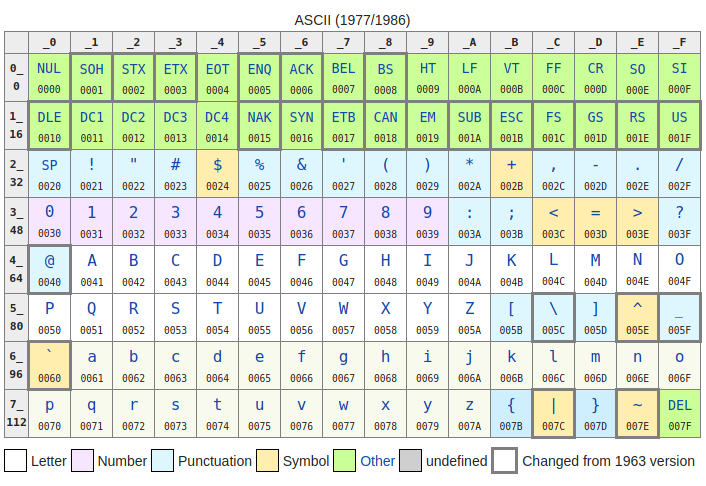
\includegraphics[width=6cm]{img/ascii.png}

  $0, \ldots, 31$ + $127$ $\rightarrow$ non-printable chars (null, new line, tab, others)
  
  $32, \ldots, 126$ $\rightarrow$ printable chars (letters, digits, punctuation, others)
  
  \medskip
  
  Extended ASCII $\rightarrow$ char encoded in 8 bit (add 128 printable chars to standard ASCII)
\end{frame}

%%%%%%%%%%%%%%%%%%%%%%%%%%%%%%%%%%%%%%%%%%%%%%%%%%%%%%%%%%%%%%%%%%%%%%%%%%%%%%%
\begin{frame}{Unicode encoding}

\centering

Obviously 128 (or 256) characters are not enough!\\
(Chinese, cyrillic, greek alphabets, emojis...)

\medskip

Different standards: UTF-8, UTF-16, UTF-32 and others

\medskip


\includegraphics[width=8cm]{img/unicode.png}

\medskip

Currently assigned "only" 137993 characters

\end{frame}

%%%%%%%%%%%%%%%%%%%%%%%%%%%%%%%%%%%%%%%%%%%%%%%%%%%%%%%%%%%%%%%%%%%%%%%%%%%%%%%
\begin{frame}{Morse code}

\centering

(Audio) character encoding scheme used in (telegraph) telecommunication.

\smallskip

Each character is encoded using a combination of short and long signal.

\medskip

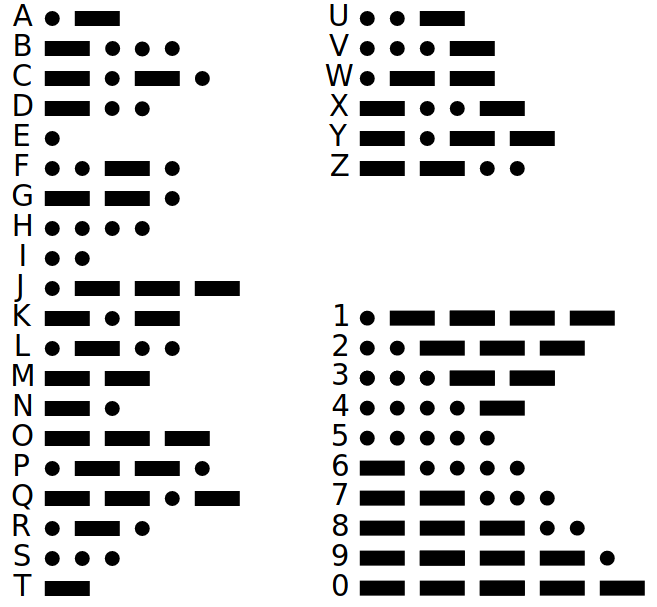
\includegraphics[width=5cm]{img/morse.png}

\end{frame}

%%%%%%%%%%%%%%%%%%%%%%%%%%%%%%%%%%%%%%%%%%%%%%%%%%%%%%%%%%%%%%%%%%%%%%%%%%%%%%%
\begin{frame}{Braille code}

\centering

(Tactile) character encoding scheme used for visually impaired people.

\smallskip

Each characted is encoded using a $2 \times 3$ rectangle with "raised dots".

\medskip

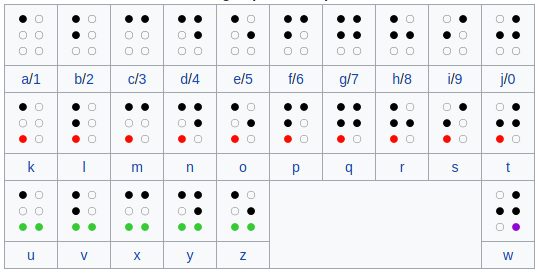
\includegraphics[width=8cm]{img/braille.png}

\end{frame}

%%%%%%%%%%%%%%%%%%%%%%%%%%%%%%%%%%%%%%%%%%%%%%%%%%%%%%%%%%%%%%%%%%%%%%%%%%%%%%%
\begin{frame}{Base64}

  \centering

  Group message in blocks of $6$ bits.

  Advantage: encode all the ASCII chars in printable chars
  
  \smallskip
  
  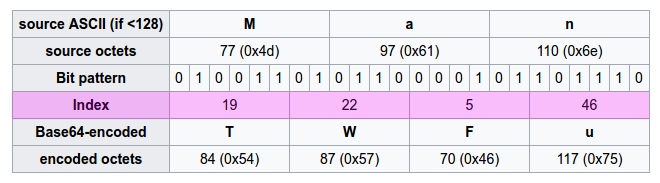
\includegraphics[width=8cm]{img/base64.png}

  \smallskip

  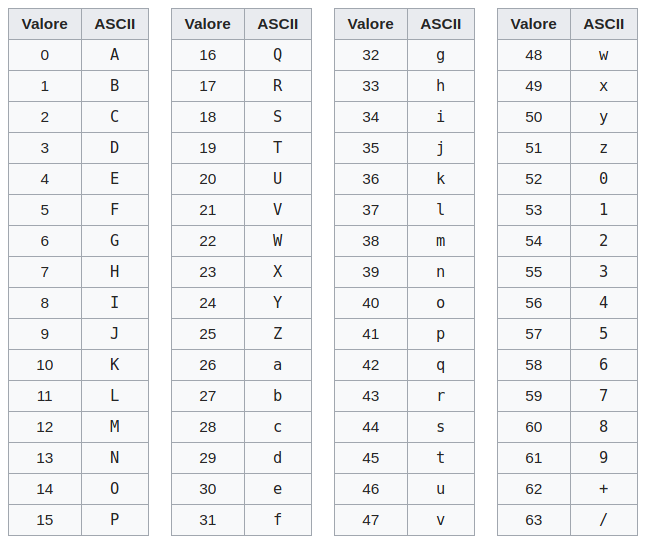
\includegraphics[width=4cm]{img/base64-2.png}

  \smallskip
  
  Message are padded with \textcolor{red}{=} (e.g. \textit{flag} $\rightarrow$ \textit{ZmxhZwo=})
  
\end{frame}

%%%%%%%%%%%%%%%%%%%%%%%%%%%%%%%%%%%%%%%%%%%%%%%%%%%%%%%%%%%%%%%%%%%%%%%%%%%%%%%
%\begin{frame}{Base65536}

%\end{frame}

%%%%%%%%%%%%%%%%%%%%%%%%%%%%%%%%%%%%%%%%%%%%%%%%%%%%%%%%%%%
\begin{frame}
  \centering
  \frametitle{Table of Contents}
  \begin{itemize}
    \item 1. Introduction
    \item 2. Message encoding
    \item 3. \textcolor{red}{Classical cryptography}
    \item 4. Symmetric-key cryptography
    \item 5. Public-key cryptography
    \item 6. Key exchange
    \item 7. Hash function
    \item 8. Steganography
  \end{itemize}  
\end{frame}
%%%%%%%%%%%%%%%%%%%%%%%%%%%%%%%%%%%%%%%%%%%%%%%%%%%%%%%%%%%%%%%%%%%%%%%%%%%%%%%
\section[Section]{Classical cryptography}
\part{Classical cryptography}

%%%%%%%%%%%%%%%%%%%%%%%%%%%%%%%%%%%%%%%%%%%%%%%%%%%%%%%%%%%%%%%%%%%%%%%%%%%%%%%
\begin{frame}{Caesar cipher}

\centering

\smallskip

Encrypt: \textcolor{red}{right shift} each letter of 3 positions

\smallskip

Decrypt: \textcolor{red}{left shift} each letter of 3 positions

\medskip

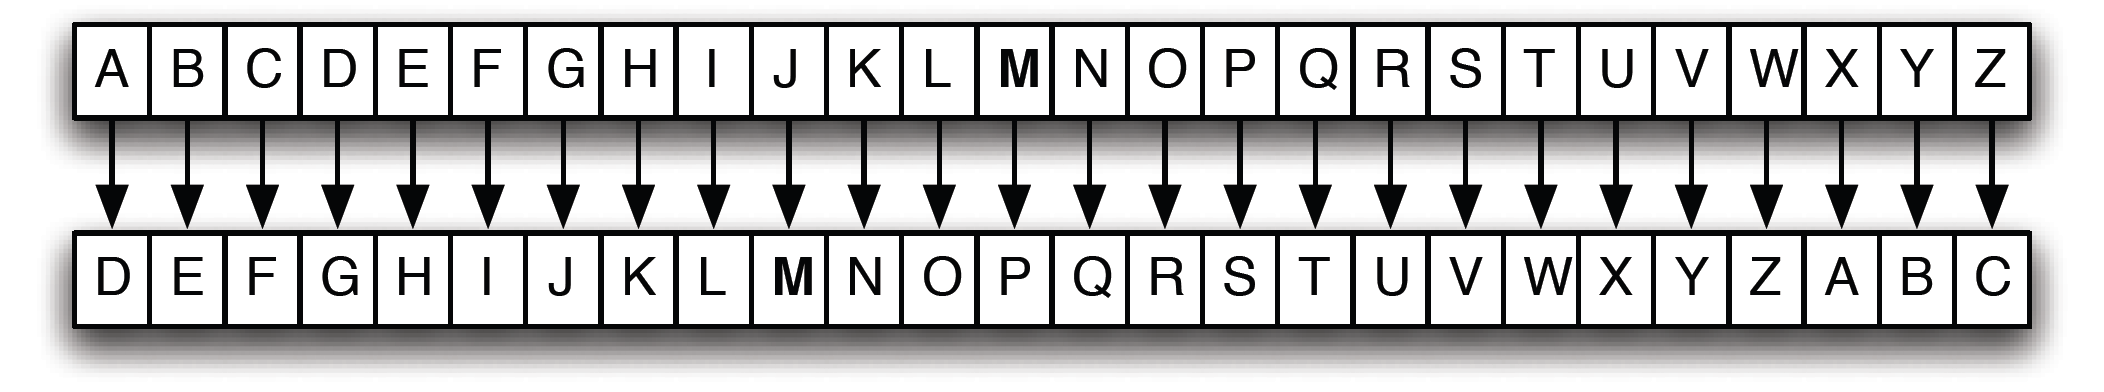
\includegraphics[width=10cm]{img/caesar-shift.png}

\medskip

General cipher: shift letter of $K$ positions

\smallskip

Attack: \textcolor{red}{bruteforce} all the possible $K$ (only $25$ values...)

\end{frame}

%%%%%%%%%%%%%%%%%%%%%%%%%%%%%%%%%%%%%%%%%%%%%%%%%%%%%%%%%%%%%%%%%%%%%%%%%%%%%%%
\begin{frame}{ROT\{13, 47\}}

\centering

\medskip

ROT13: Caesar cipher with $K = 13$ on alphabetic dictionary

ROT47: Caesar cipher with $K = 47$ on printable ASCII chars (33 - 126).

\medskip

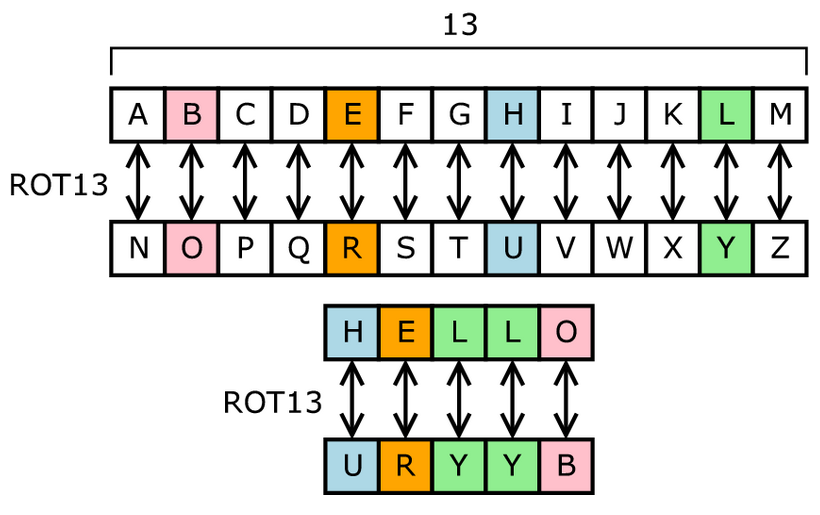
\includegraphics[width=8cm]{img/ROT13.png}

\medskip

Why $K = 13$ (or $K = 47$)? Because \textcolor{red}{Encrypt = Decrypt}

\end{frame}

%%%%%%%%%%%%%%%%%%%%%%%%%%%%%%%%%%%%%%%%%%%%%%%%%%%%%%%%%%%%%%%%%%%%%%%%%%%%%%%
\begin{frame}{Classical ciphers}

\textbf{Substitution ciphers}

\phantom{pad}- Monoalphabetic ciphers: \textcolor{red}{$C_{new} = P[C_{old}]$} (Where $P$ is a dictionary permutation)

\smallskip

\phantom{pad}(ROT-K is a monoalphabetic cipher with $P$ is a cyclic rotation)

\smallskip

\phantom{pad}- Polialphabetic ciphers: \textcolor{red}{multiple substitution} alphabets 

\phantom{pad}(more than one dictionary permutation)

\smallskip

\textbf{Transposition ciphers}

\phantom{pad}Encryption systems where the \textcolor{red}{positions} held by units of plaintext 

\phantom{pad}(characters or groups of characters) \textcolor{red}{are shifted} according to a regular system.

\smallskip

E.g. We want to encrypt the message \textit{WE ARE DISCOVERED. FLEE AT ONCE} using the \textbf{route cipher}:

Grid: 

\centerline{\texttt{W R I O R F E O E}}
\centerline{\texttt{E E S V E L A N J}}
\centerline{\texttt{A D C E D E T C X}}

Cipher text: \textit{EJXCTEDECDAEWRIORFEONALEVSE}

\end{frame}
%%%%%%%%%%%%%%%%%%%%%%%%%%%%%%%%%%%%%%%%%%%%%%%%%%%%%%%%%%%%%%%%%%%%%%%%%%%%%%%
\begin{frame}{Polialphabetic substituion cipher: Vigenère}
  
The problem with monoalphabetic ciphers is that each character of the alphabet is replaced with always the same character in the ciphertext.

\smallskip

What can we do to solve this weakness? \textcolor{red}{Stack more ciphers}!

The Vigenère cipher is basically a \textbf{sequence of Caesar ciphers with different shifts}.

\smallskip

  \begin{columns}
  \begin{column}{0.4\textwidth}

    \centerline{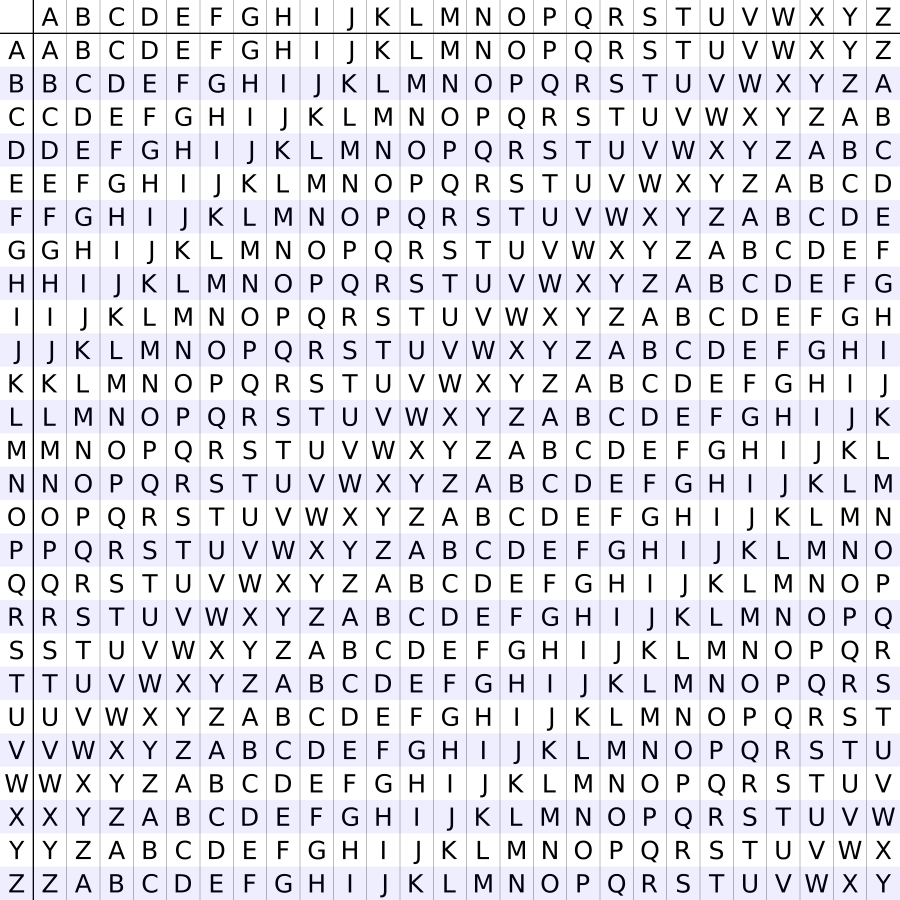
\includegraphics[width=4cm]{img/VigenereTable.png}}

    This table is called \textcolor{red}{Vigenère table}.
    
    It contains all the Caesar ciphers. 

  \end{column}
  \begin{column}{0.6\textwidth}


    Encryption is performed character-by-character by accessing the cell of the table within the row corresponding to the current key letter and column to the plaintext letter.

    Decryption works in the same way of the encryption but we use a transposed Vigenère table.

    This simple technique earned the name of \textcolor{red}{the indecipherable cipher}, and resisted attacks for over 3 centuries (1553-1863)!

  \end{column}
  \end{columns}



\end{frame}
%%%%%%%%%%%%%%%%%%%%%%%%%%%%%%%%%%%%%%%%%%%%%%%%%%%%%%%%%%%%%%%%%%%%%%%%%%%%%%%
\begin{frame}{Vigenère cipher: an example}
  
  We want to encrypt the message \texttt{THIS IS AN EXAMPLE} with the key \texttt{SECRET}

  \medskip
  
  First of all, we repeat the key until it has the same length of the plaintext: \\

  \medskip
  
  $m =$ \texttt{THISISANEXAMPLE}\\
  $k =$ \texttt{SECRETSECRETSEC}\\

  \medskip
  
  In our example, the first letter of the plaintext is $T$ and the first of the key is $S$, so we access the row $S$ and column $T$, which yields $L$. 
  
  And so on until the end of the message:\\

  \medskip
  
  $c =$ \texttt{LLKJMLSRGOEFHPG}

\end{frame}
%%%%%%%%%%%%%%%%%%%%%%%%%%%%%%%%%%%%%%%%%%%%%%%%%%%%%%%%%%%%%%%%%%%%%%%%%%%%%%%
\begin{frame}{Transposition cipher: an example}

The plaintext is written in a rectangular grid and then the columns are reshuffled, the encryption key is the \textcolor{red}{column permutation}

\medskip

$m =$ \texttt{THIS IS AN EXAMPLE}\\
$k =$ \texttt{\{4, 2, 1, 3\}}

\medskip

\centerline{\texttt{T H I S  \phantom{-------------------->} S H T I}}
\centerline{\texttt{I S A N  \phantom{---}Reorder columns\phantom{---} N S I A}}
\centerline{\texttt{E X A M  \phantom{---}-------------->\phantom{---} M X E A}}
\centerline{\texttt{P L E =  \phantom{-------------------->} = L P E}}

\medskip

$c =$ \texttt{SHTINSIAMXEA=LPE}

\medskip

To recover the original message, just write the ciphertext in a grid again and apply the inverse permutation of columns

\end{frame}
%%%%%%%%%%%%%%%%%%%%%%%%%%%%%%%%%%%%%%%%%%%%%%%%%%%%%%%%%%%%%%%%%%%%%%%%%%%%%%%
\begin{frame}{dcode.fr}

\centering

\href{https://www.dcode.fr/tools-list}{https://www.dcode.fr/tools-list}

\medskip

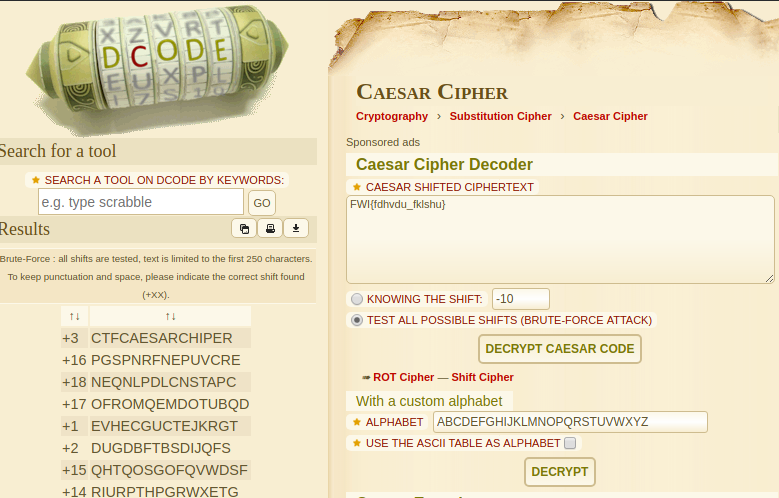
\includegraphics[width=8cm]{img/dcode.png}

\medskip

\textcolor{red}{Almost} all possible classic ciphers (old and new), encoder/decoder, ...

\end{frame}
%%%%%%%%%%%%%%%%%%%%%%%%%%%%%%%%%%%%%%%%%%%%%%%%%%%%%%%%%%%%%%%%%%%%%%%%%%%%%%%
\begin{frame}{Cryptanalysis}

Often the vulnerability is not in the algorithm but in \textcolor{red}{its application}...

\begin{itemize}
  \item Bad use of the key (too short, reused, bad generated, ...)
  \item Messages use a poorly distributed dictionary
  \item We know the message format (e.g.: \textsc{flag\{\ldots\}})
\end{itemize}

\medskip

In particular we talk about \textcolor{red}{statistical cryptanalysis} when we force the cipher not from algorithmic point of view but from statistical one

\medskip

For example in english the character E has a frequency of 12.02\% while Z only 0.07\%

\medskip

Useful tool (for substitution ciphers): \href{https://quipqiup.com}{https://quipqiup.com}

\medskip

\centering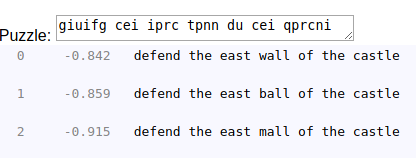
\includegraphics[width=5cm]{img/quipqiup.png}
  
\end{frame}
%%%%%%%%%%%%%%%%%%%%%%%%%%%%%%%%%%%%%%%%%%%%%%%%%%%%%%%%%%%%%%%%%%%%%%%%%%%%%%%

\begin{frame}{Attack models}

Classification of cryptographic attacks:

\medskip

\begin{itemize}
  \item \textcolor{red}{Ciphertext-only} attack: access only to the ciphertext, and has no access to the plaintext
  \medskip
  \item \textcolor{red}{Known-plaintext} attack: access to at least a limited number of pairs of plaintext and the corresponding enciphered text
  \medskip
  \item \textcolor{red}{Chosen plaintext} attack: able to choose a number of plaintexts to be enciphered and have access to the resulting ciphertext (encrypt oracle)
  \medskip
  \item \textcolor{red}{Chosen ciphertext} attack: able to choose arbitrary ciphertext and have access to plaintext decrypted from it (decrypt oracle) 
  \medskip
  \item \textcolor{red}{Side-channel} attack: use of other informations to break the cipher (time, sound, power, error, ...).
\end{itemize}
  
\end{frame}
%%%%%%%%%%%%%%%%%%%%%%%%%%%%%%%%%%%%%%%%%%%%%%%%%%%%%%%%%%%%%%%%%%%%%%%%%%%%%%%

%%%%%%%%%%%%%%%%%%%%%%%%%%%%%%%%%%%%%%%%%%%%%%%%%%%%%%%%%%%
\begin{frame}
  \centering
  \frametitle{Table of Contents}
  \begin{itemize}
    \item 1. Introduction
    \item 2. Message encoding
    \item 3. Classical cryptography
    \item 4. \textcolor{red}{Symmetric-key cryptography}
    \item 5. Public-key cryptography
    \item 6. Key exchange
    \item 7. Hash function
    \item 8. Steganography
  \end{itemize}  
\end{frame}
%%%%%%%%%%%%%%%%%%%%%%%%%%%%%%%%%%%%%%%%%%%%%%%%%%%%%%%%%%%%%%%%%%%%%%%%%%%%%%%
\section[Section]{Symmetric-key cryptography}
\part{Symmetric-key cryptography}

%%%%%%%%%%%%%%%%%%%%%%%%%%%%%%%%%%%%%%%%%%%%%%%%%%%%%%%%%%%%%%%%%%%%%%%%%%%%%%%
\begin{frame}{Symmetric-key cryptography}

\end{frame}

%%%%%%%%%%%%%%%%%%%%%%%%%%%%%%%%%%%%%%%%%%%%%%%%%%%%%%%%%%%%%%%%%%%%%%%%%%%%%%%
\begin{frame}{Shannon principle}

\end{frame}

%%%%%%%%%%%%%%%%%%%%%%%%%%%%%%%%%%%%%%%%%%%%%%%%%%%%%%%%%%%%%%%%%%%%%%%%%%%%%%%
\begin{frame}{XOR cipher}

\end{frame}

%%%%%%%%%%%%%%%%%%%%%%%%%%%%%%%%%%%%%%%%%%%%%%%%%%%%%%%%%%%%%%%%%%%%%%%%%%%%%%%
\begin{frame}{One-time pad}

\end{frame}

%%%%%%%%%%%%%%%%%%%%%%%%%%%%%%%%%%%%%%%%%%%%%%%%%%%%%%%%%%%%%%%%%%%%%%%%%%%%%%%
\begin{frame}{Many-time pad}

\end{frame}

%%%%%%%%%%%%%%%%%%%%%%%%%%%%%%%%%%%%%%%%%%%%%%%%%%%%%%%%%%%%%%%%%%%%%%%%%%%%%%%
\begin{frame}{XorTool}

\end{frame}

%%%%%%%%%%%%%%%%%%%%%%%%%%%%%%%%%%%%%%%%%%%%%%%%%%%%%%%%%%%%%%%%%%%%%%%%%%%%%%%
\begin{frame}{Block vs Stream ciphers}

\end{frame}

%%%%%%%%%%%%%%%%%%%%%%%%%%%%%%%%%%%%%%%%%%%%%%%%%%%%%%%%%%%%%%%%%%%%%%%%%%%%%%%
\begin{frame}{DES}

\end{frame}

%%%%%%%%%%%%%%%%%%%%%%%%%%%%%%%%%%%%%%%%%%%%%%%%%%%%%%%%%%%%%%%%%%%%%%%%%%%%%%%
\begin{frame}{AES}

\end{frame}

%%%%%%%%%%%%%%%%%%%%%%%%%%%%%%%%%%%%%%%%%%%%%%%%%%%%%%%%%%%%%%%%%%%%%%%%%%%%%%%
\begin{frame}{Padding a message (PKCS\#5 \& PKCS\#7)}

% \centering

How to handle messages of length not multiple of the block size?

\smallskip

Idea: append "some chars" to the message

\bigskip

\textbf{PKCS\#5}:

\textit{The padding string PS shall consist of $8 - (||M|| \mod 8)$ octets all having value $8 - (||M|| \mod 8).$}

\bigskip

\textbf{PKCS\#7}:

\textit{For such algorithms, the method shall be to pad the input at the trailing end with $k - (l \mod k)$ octets all having value $k - (l \mod k)$, where $l$ is the length of the input.}

\bigskip

Why $8 - (||M|| \mod 8)$ and not $(||M|| \mod 8)$?
\end{frame}

%%%%%%%%%%%%%%%%%%%%%%%%%%%%%%%%%%%%%%%%%%%%%%%%%%%%%%%%%%%%%%%%%%%%%%%%%%%%%%%
\begin{frame}{Block cipher mode of operation}

\end{frame}

%%%%%%%%%%%%%%%%%%%%%%%%%%%%%%%%%%%%%%%%%%%%%%%%%%%%%%%%%%%%%%%%%%%%%%%%%%%%%%%
\begin{frame}{ECB (Electronic Codebook)}

\centering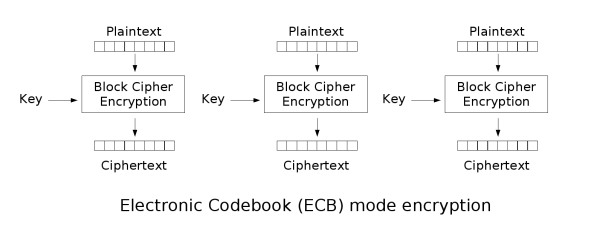
\includegraphics[width=9cm]{img/ECB.png}

\medskip

\centering

$C_i = f(M_i, Key)$

\end{frame}

%%%%%%%%%%%%%%%%%%%%%%%%%%%%%%%%%%%%%%%%%%%%%%%%%%%%%%%%%%%%%%%%%%%%%%%%%%%%%%%
\begin{frame}{How to break ECB (padding-oracle attack)}

\end{frame}

%%%%%%%%%%%%%%%%%%%%%%%%%%%%%%%%%%%%%%%%%%%%%%%%%%%%%%%%%%%%%%%%%%%%%%%%%%%%%%%
\begin{frame}{CBC (Cipher Block Chaining)}

\centering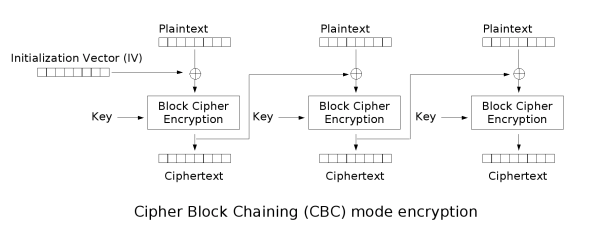
\includegraphics[width=9cm]{img/CBC.png}

\medskip

\centering

$C_i = f(M_i \oplus IV_{i}, Key)$

\medskip

$IV_0 = $ given in input (randomly generated)

\medskip

$IV_{i+1} = C_i$

\end{frame}

%%%%%%%%%%%%%%%%%%%%%%%%%%%%%%%%%%%%%%%%%%%%%%%%%%%%%%%%%%%%%%%%%%%%%%%%%%%%%%%
\begin{frame}{How to break CBC (bit-flipping attack)}

\end{frame}

%%%%%%%%%%%%%%%%%%%%%%%%%%%%%%%%%%%%%%%%%%%%%%%%%%%%%%%%%%%%%%%%%%%%%%%%%%%%%%%
%\begin{frame}{Stream ciphers (Salsa \& Cha-Cha)}

%\end{frame}

%%%%%%%%%%%%%%%%%%%%%%%%%%%%%%%%%%%%%%%%%%%%%%%%%%%%%%%%%%%
\begin{frame}
  \centering
  \frametitle{Table of Contents}
  \begin{itemize}
    \item 1. Introduction
    \item 2. Message encoding
    \item 3. Classical cryptography
    \item 4. Symmetric-key cryptography
    \item 5. \textcolor{red}{Public-key cryptography}
    \item 6. Key exchange
    \item 7. Hash function
    \item 8. Steganography
  \end{itemize}  
\end{frame}
%%%%%%%%%%%%%%%%%%%%%%%%%%%%%%%%%%%%%%%%%%%%%%%%%%%%%%%%%%%%%%%%%%%%%%%%%%%%%%%
\section{Public-key cryptography}
\part{Public-key cryptography}

%%%%%%%%%%%%%%%%%%%%%%%%%%%%%%%%%%%%%%%%%%%%%%%%%%%%%%%%%%%%%%%%%%%%%%%%%%%%%%%
\begin{frame}{Public-key cryptography}

\end{frame}

%%%%%%%%%%%%%%%%%%%%%%%%%%%%%%%%%%%%%%%%%%%%%%%%%%%%%%%%%%%%%%%%%%%%%%%%%%%%%%%
\begin{frame}{Modular arithmetic}

\end{frame}

%%%%%%%%%%%%%%%%%%%%%%%%%%%%%%%%%%%%%%%%%%%%%%%%%%%%%%%%%%%%%%%%%%%%%%%%%%%%%%%
\begin{frame}{RSA}

\end{frame}

%%%%%%%%%%%%%%%%%%%%%%%%%%%%%%%%%%%%%%%%%%%%%%%%%%%%%%%%%%%%%%%%%%%%%%%%%%%%%%%
\begin{frame}{An example...}

\end{frame}

%%%%%%%%%%%%%%%%%%%%%%%%%%%%%%%%%%%%%%%%%%%%%%%%%%%%%%%%%%%%%%%%%%%%%%%%%%%%%%%
\begin{frame}{How to choose parameters}

\end{frame}

%%%%%%%%%%%%%%%%%%%%%%%%%%%%%%%%%%%%%%%%%%%%%%%%%%%%%%%%%%%%%%%%%%%%%%%%%%%%%%%
\begin{frame}{Break RSA (online approach)}

\end{frame}

%%%%%%%%%%%%%%%%%%%%%%%%%%%%%%%%%%%%%%%%%%%%%%%%%%%%%%%%%%%%%%%%%%%%%%%%%%%%%%%
\begin{frame}{Break RSA (offline approach)}

\end{frame}

%%%%%%%%%%%%%%%%%%%%%%%%%%%%%%%%%%%%%%%%%%%%%%%%%%%%%%%%%%%%%%%%%%%%%%%%%%%%%%%
\begin{frame}{Break RSA (online approach)}

\end{frame}

%%%%%%%%%%%%%%%%%%%%%%%%%%%%%%%%%%%%%%%%%%%%%%%%%%%%%%%%%%%
\begin{frame}
  \centering
  \frametitle{Table of Contents}
  \begin{itemize}
    \item 1. Introduction
    \item 2. Message encoding
    \item 3. Classical cryptography
    \item 4. Symmetric-key cryptography
    \item 5. Public-key cryptography
    \item 6. \textcolor{red}{Key exchange}
    \item 7. Hash function
    \item 8. Steganography
  \end{itemize}  
\end{frame}
%%%%%%%%%%%%%%%%%%%%%%%%%%%%%%%%%%%%%%%%%%%%%%%%%%%%%%%%%%%%%%%%%%%%%%%%%%%%%%%
\section{Key exchange}
\part{Key exchange}

%%%%%%%%%%%%%%%%%%%%%%%%%%%%%%%%%%%%%%%%%%%%%%%%%%%%%%%%%%%%%%%%%%%%%%%%%%%%%%%
\begin{frame}{Key exchange}

\end{frame}

%%%%%%%%%%%%%%%%%%%%%%%%%%%%%%%%%%%%%%%%%%%%%%%%%%%%%%%%%%%%%%%%%%%%%%%%%%%%%%%
\begin{frame}{Diffie-Hellman key exchange}

\end{frame}

%%%%%%%%%%%%%%%%%%%%%%%%%%%%%%%%%%%%%%%%%%%%%%%%%%%%%%%%%%%%%%%%%%%%%%%%%%%%%%%
\begin{frame}{A man-in-the-middle attack to DH}

\end{frame}

%%%%%%%%%%%%%%%%%%%%%%%%%%%%%%%%%%%%%%%%%%%%%%%%%%%%%%%%%%%
\begin{frame}
  \centering
  \frametitle{Table of Contents}
  \begin{itemize}
    \item 1. Introduction
    \item 2. Message encoding
    \item 3. Classical cryptography
    \item 4. Symmetric-key cryptography
    \item 5. Public-key cryptography
    \item 6. Key exchange
    \item 7. \textcolor{red}{Hash function}
    \item 8. Steganography
  \end{itemize}  
\end{frame}
%%%%%%%%%%%%%%%%%%%%%%%%%%%%%%%%%%%%%%%%%%%%%%%%%%%%%%%%%%%%%%%%%%%%%%%%%%%%%%%
\section[Section]{Hash function}
\part{Hash function}

%%%%%%%%%%%%%%%%%%%%%%%%%%%%%%%%%%%%%%%%%%%%%%%%%%%%%%%%%%%%%%%%%%%%%%%%%%%%%%%
\begin{frame}{Hash function}

\end{frame}

%%%%%%%%%%%%%%%%%%%%%%%%%%%%%%%%%%%%%%%%%%%%%%%%%%%%%%%%%%%%%%%%%%%%%%%%%%%%%%%
\begin{frame}{Why hash}

\end{frame}

%%%%%%%%%%%%%%%%%%%%%%%%%%%%%%%%%%%%%%%%%%%%%%%%%%%%%%%%%%%%%%%%%%%%%%%%%%%%%%%
\begin{frame}{How to store passwords}

\end{frame}

%%%%%%%%%%%%%%%%%%%%%%%%%%%%%%%%%%%%%%%%%%%%%%%%%%%%%%%%%%%%%%%%%%%%%%%%%%%%%%%
\begin{frame}{How to store passwords$^2$}

\end{frame}

%%%%%%%%%%%%%%%%%%%%%%%%%%%%%%%%%%%%%%%%%%%%%%%%%%%%%%%%%%%%%%%%%%%%%%%%%%%%%%%
\begin{frame}{How to \textcolor{red}{(not)} store passwords}

\end{frame}

%%%%%%%%%%%%%%%%%%%%%%%%%%%%%%%%%%%%%%%%%%%%%%%%%%%%%%%%%%%%%%%%%%%%%%%%%%%%%%%
\begin{frame}{Proof of Work}

\end{frame}

%%%%%%%%%%%%%%%%%%%%%%%%%%%%%%%%%%%%%%%%%%%%%%%%%%%%%%%%%%%%%%%%%%%%%%%%%%%%%%%
\begin{frame}{MD5}

\end{frame}

%%%%%%%%%%%%%%%%%%%%%%%%%%%%%%%%%%%%%%%%%%%%%%%%%%%%%%%%%%%%%%%%%%%%%%%%%%%%%%%
\begin{frame}{SHA\{0, 1, 2\}}

\end{frame}

%%%%%%%%%%%%%%%%%%%%%%%%%%%%%%%%%%%%%%%%%%%%%%%%%%%%%%%%%%%%%%%%%%%%%%%%%%%%%%%
\begin{frame}{Finding collision}

\end{frame}

%%%%%%%%%%%%%%%%%%%%%%%%%%%%%%%%%%%%%%%%%%%%%%%%%%%%%%%%%%%%%%%%%%%%%%%%%%%%%%%
\begin{frame}{Reverse an hash function (online approach)}

\end{frame}

%%%%%%%%%%%%%%%%%%%%%%%%%%%%%%%%%%%%%%%%%%%%%%%%%%%%%%%%%%%%%%%%%%%%%%%%%%%%%%%
\begin{frame}{Reverse an hash function (offline approach)}

\end{frame}

%%%%%%%%%%%%%%%%%%%%%%%%%%%%%%%%%%%%%%%%%%%%%%%%%%%%%%%%%%%%%%%%%%%%%%%%%%%%%%%
\begin{frame}{fcrackzip}

\end{frame}

%%%%%%%%%%%%%%%%%%%%%%%%%%%%%%%%%%%%%%%%%%%%%%%%%%%%%%%%%%%%%%%%%%%%%%%%%%%%%%%
\begin{frame}{JohnTheRipper}

\end{frame}

%%%%%%%%%%%%%%%%%%%%%%%%%%%%%%%%%%%%%%%%%%%%%%%%%%%%%%%%%%%%%%%%%%%%%%%%%%%%%%%
\begin{frame}{Hashcat}

\end{frame}


%%%%%%%%%%%%%%%%%%%%%%%%%%%%%%%%%%%%%%%%%%%%%%%%%%%%%%%%%%%
\begin{frame}
  \centering
  \frametitle{Table of Contents}
  \begin{itemize}
    \item 1. Introduction
    \item 2. Message encoding
    \item 3. Classical cryptography
    \item 4. Symmetric-key cryptography
    \item 5. Public-key cryptography
    \item 6. Key exchange
    \item 7. Hash function
    \item 8. \textcolor{red}{Steganography}
  \end{itemize}  
\end{frame}
%%%%%%%%%%%%%%%%%%%%%%%%%%%%%%%%%%%%%%%%%%%%%%%%%%%%%%%%%%%%%%%%%%%%%%%%%%%%%%%
\section[Section]{Steganography}
\part{Steganography}

%%%%%%%%%%%%%%%%%%%%%%%%%%%%%%%%%%%%%%%%%%%%%%%%%%%%%%%%%%%%%%%%%%%%%%%%%%%%%%%
\begin{frame}{Steganography}

\end{frame}

%%%%%%%%%%%%%%%%%%%%%%%%%%%%%%%%%%%%%%%%%%%%%%%%%%%%%%%%%%%%%%%%%%%%%%%%%%%%%%%
\begin{frame}{File stego (file, binwalk, exiftool, strings)}

\end{frame}

%%%%%%%%%%%%%%%%%%%%%%%%%%%%%%%%%%%%%%%%%%%%%%%%%%%%%%%%%%%%%%%%%%%%%%%%%%%%%%%
\begin{frame}{Image stego}

\end{frame}

%%%%%%%%%%%%%%%%%%%%%%%%%%%%%%%%%%%%%%%%%%%%%%%%%%%%%%%%%%%%%%%%%%%%%%%%%%%%%%%
\begin{frame}{Layer stego}

\end{frame}

%%%%%%%%%%%%%%%%%%%%%%%%%%%%%%%%%%%%%%%%%%%%%%%%%%%%%%%%%%%%%%%%%%%%%%%%%%%%%%%
\begin{frame}{Audio stego}

\end{frame}

%%%%%%%%%%%%%%%%%%%%%%%%%%%%%%%%%%%%%%%%%%%%%%%%%%%%%%%%%%%%%%%%%%%%%%%%%%%%%%%
\begin{frame}{Morse code}

\end{frame}

%%%%%%%%%%%%%%%%%%%%%%%%%%%%%%%%%%%%%%%%%%%%%%%%%%%%%%%%%%%%%%%%%%%%%%%%%%%%%%%
\begin{frame}{Spectography analysis (Audacity)}

\end{frame}

%%%%%%%%%%%%%%%%%%%%%%%%%%%%%%%%%%%%%%%%%%%%%%%%%%%%%%%%%%%%%%%%%%%%%%%%%%%%%%%
\begin{frame}{AudioStego}

\end{frame}

%%%%%%%%%%%%%%%%%%%%%%%%%%%%%%%%%%%%%%%%%%%%%%%%%%%%%%%%%%%%%%%%%%%%%%%%%%%%%%%
\begin{frame}{DeepSound}

\end{frame}
%%%%%%%%%%%%%%%%%%%%%%%%%%%%%%%%%%%%%%%%%%%%%%%%%%%%%%%%%%%%%%%%%%%%%%%%%%%%%%%


\end{document}
